\begin{frame}
  \frametitle{Conjetura de los espejos.}
  Supongamos que tenemos una colección $F$ de segmentos de lineas cerrados
  y ajenos que representan una colección de espejos que reflejan luz en ambos
  lados, y sea $p$ un punto en el plano.
  \begin{figure}
    \centering
    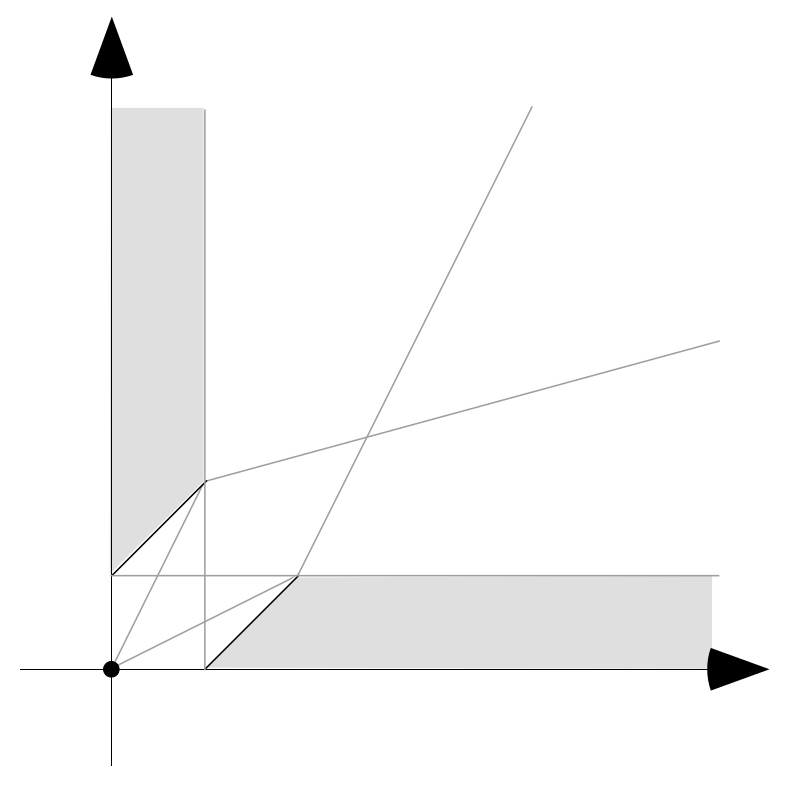
\includegraphics[width=.25 \paperwidth]{./images/Espejos.png}
    %\caption*{.}
  \end{figure}
  Supongamos que tenemos una lámpara colocada en $p$ que emite luz a su
  alrededor. Un región $S$ del plano con interior no vacio será llamada la sombra
  de $F$, si todo punto en el interior de $S$ no es iluminado por al menos un rayo
  de luz que llege a él ya sea directamente de $p$, o despues de reflejarse varias
  veces en algunos espejos de $F$.\newline

  .
\end{frame}

\begin{frame}
  \frametitle{Conjetura de los espejos.}
  \begin{conjetura}
    Sea F una familia de $n$ espejos finitos y $p$ un punto que no
    está en la recta generada por alguno de los espejos en $F$. Entonces siempre
    se genera una sombra de área infinita en el plano.
  \end{conjetura}
  \begin{figure}
    \centering
    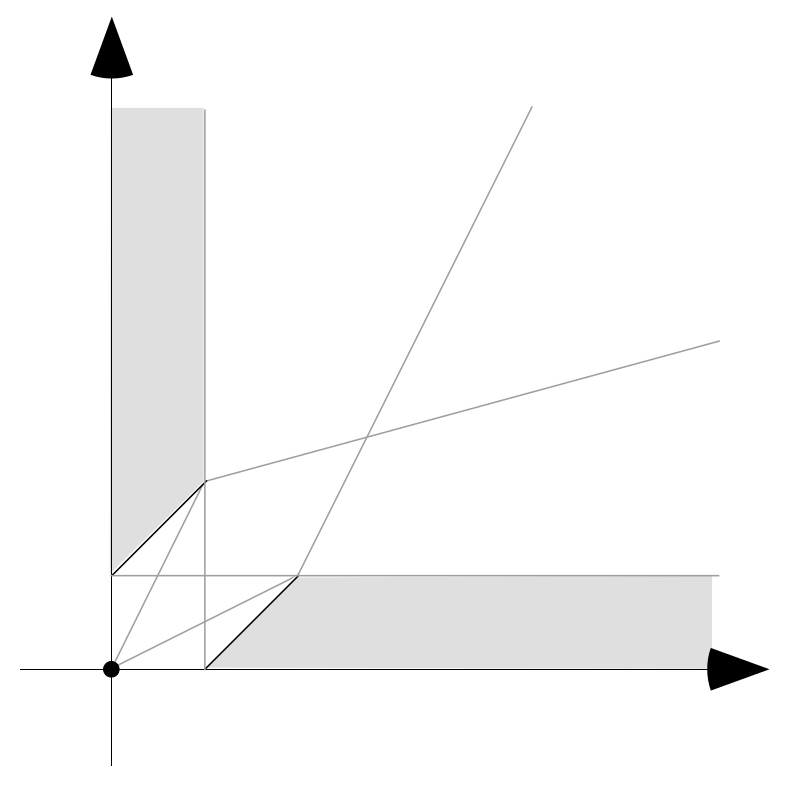
\includegraphics[width=.25 \paperwidth]{./images/Espejos.png}
    %\caption*{.}
  \end{figure}
\end{frame}

\begin{frame}
  \frametitle{Conjetura de los espejos.}
  \begin{conjetura}
    Sea F una familia de $n$ espejos finitos y $p$ un punto que no
    está en la recta generada por alguno de los espejos en $F$. Entonces siempre
    se genera una sombra de área infinita en el plano.
  \end{conjetura}
  \begin{figure}
    \centering
    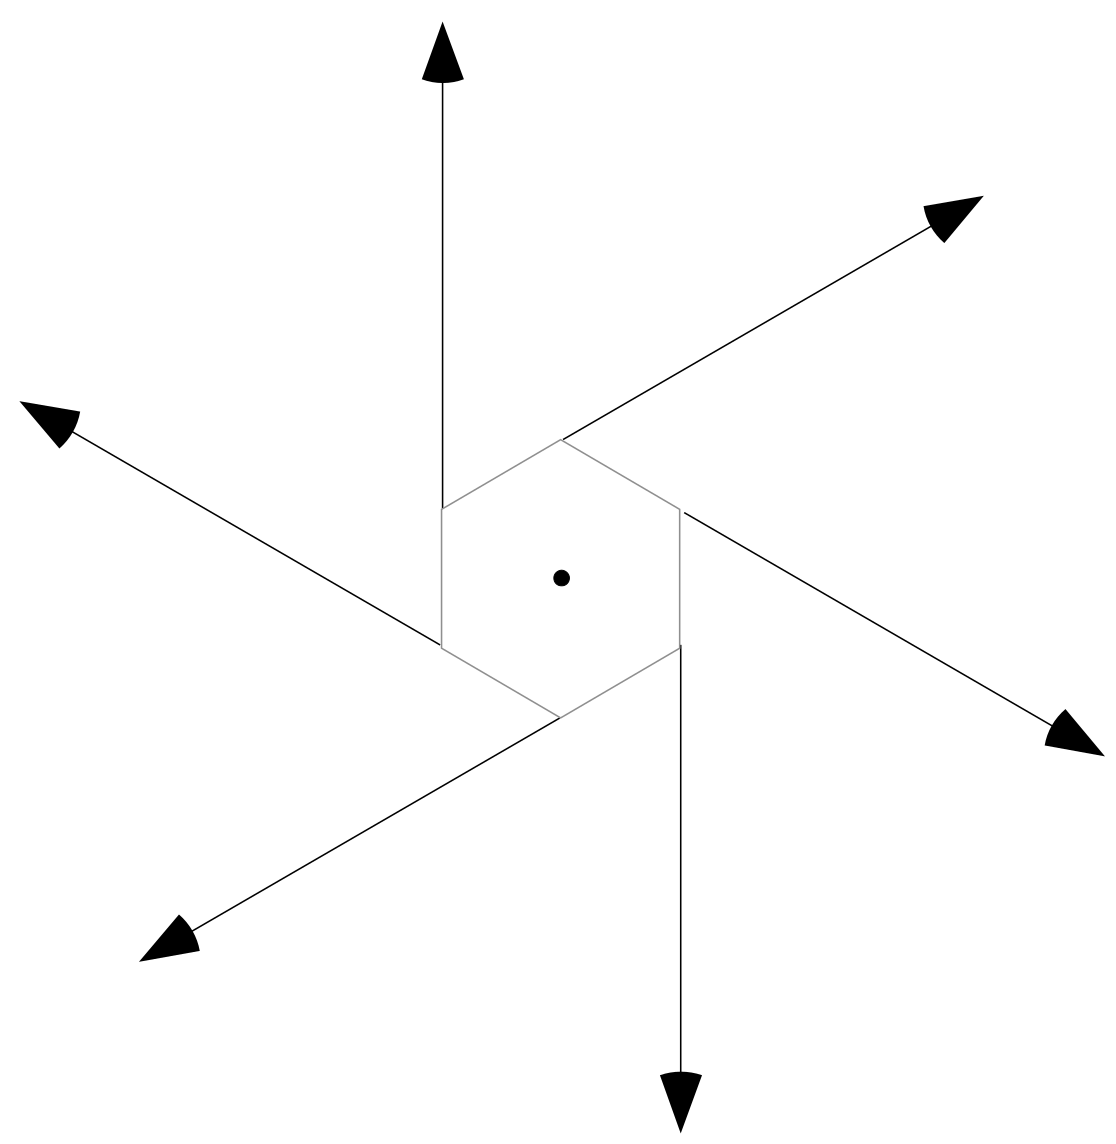
\includegraphics[width=.25 \paperwidth]{./images/EspejosInfinitos.png}
    %\caption*{.}
  \end{figure}
\end{frame}
